\chapter{Configurazione dei progetti RoboCheckers in Eclipse}
Questa appendice illustra brevemente come configurare correttamente
Eclipse e scaricare i sorgenti dei due progetti sviluppati.
Si d� come presupporto di avere gi� installato Eclipse con il
plugin per la gestione dell'SVN\footnote{Nel caso in cui non fosse ancora
stato installato il plugin per gestire l'SVN riferirsi al paragrafo
\ref{sec:checkoutsvn}}.
\section{Installazione di Lejos}
Il primo passo per la configurazione dei progetti consiste nell'installazione
di Lejos.
L'installazione � molto semplice, una volta scaricato il setup dal sito
ufficiale \url{http://lejos.sourceforge.net/} � sufficiente seguire il wizard
fino alla fine, l'unica cosa importante da fare � ricordarsi la cartella in cui
lo si decide di installare in quanto sar� necessaria in seguito.
\section{Installazione del Plugin di Lejos}
Dopo aver installato Lejos � possibile installare il Plugin per Eclipse cos� da
poter compilare e caricare i programmi sull'\texttt{NXT} direttamente da
Eclipse. Per farlo, selezionare il men� \texttt{Help}$\to$\texttt{Software Updates} e nella sezione
\emph{Available Software} selezionare \texttt{Add Site}.\\
	\begin{figure}
		\begin{center}
			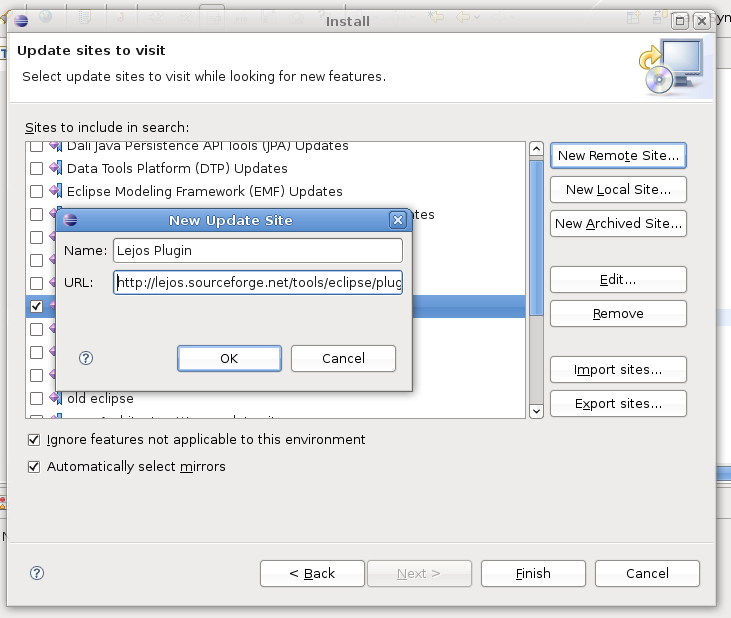
\includegraphics[scale=0.45]{img/lejosplugin01.png}
			\caption{Installazione del plugin di Lejos \label{fig:lejosplugin01}}
		\end{center}
	\end{figure}
\paragraph{}
Nella finestra di dialogo digitare
\url{http://lejos.sourceforge.net/tools/eclipse/plugin/nxj/} e premere \texttt{OK}.\\
Espandere la voce appena aggiunta e selezionare tutti i sotto-elementi,
successivamente premere \texttt{Install} e procedere con l'installazione.
	\begin{figure}
		\begin{center}
			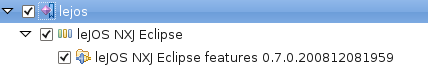
\includegraphics[scale=0.6]{img/lejosplugin02.png}
			\caption{Installazione del plugin di Lejos \label{fig:lejosplugin02}}
		\end{center}
	\end{figure}
\paragraph{}
Una volta riavviato Eclipse, � necessario configurare il plugin indicando la
cartella dove � stato installato Lejos. Da
\texttt{Window}$\to$\texttt{Preferences} selezionere \texttt{Lejos NXT} e
completare il campo \texttt{NXT\_HOME} con il percorso della cartella dove avete
installato, al passo precedente, \texttt{Lejos}.
	\begin{figure}
		\begin{center}
			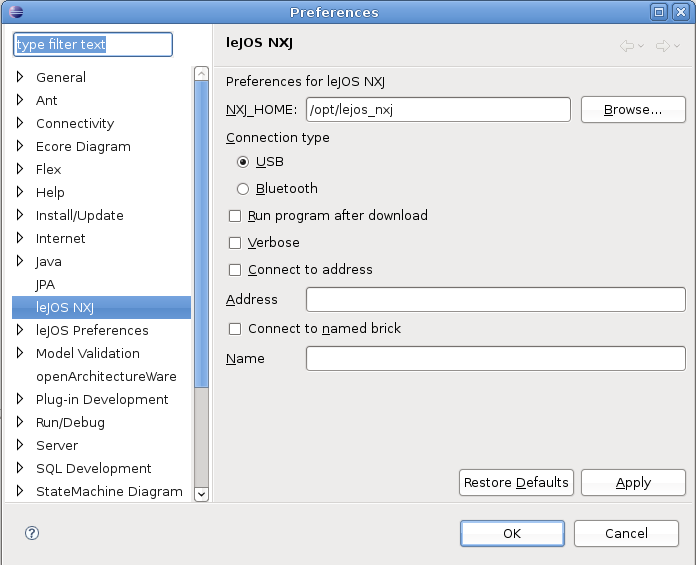
\includegraphics[scale=0.45]{img/lejosplugin03.png}
			\caption{Configurazione del plugin di Lejos \label{fig:lejosplugin03}}
		\end{center}
	\end{figure}

\section{Configurazione delle variabili d'ambiente}
A questo punto, prima di procedere con il download dei sorgenti, � ancora
necessario un altro piccolo passo per la configurazione dell'ambiente. Questo
si � reso necessario perch� \emph{Lejos} sui vari sistemi operativi � installato
in posizioni diverse quindi al fine di rendere il progetto generico � necessario
specificare alcune variabili per la configurazione corretta del Classpath di
Java.\\
Da \texttt{Window}$\to$\texttt{Preferences} selezionere la sezione
\emph{Java}$\to$\emph{Build Path}$\to$\emph{Classpath Variable},
selezionare quindi \texttt{New}. Nella finestra che appare completare il
campo \texttt{Name} con \texttt{NXJ\_CLASSES} e quindi selezionare
\texttt{File} e selezionare il file \emph{classes.jar} che si trova
all'interno della cartella lib dell'installazione di \emph{Lejos}.\\
	\begin{figure}
		\begin{center}
			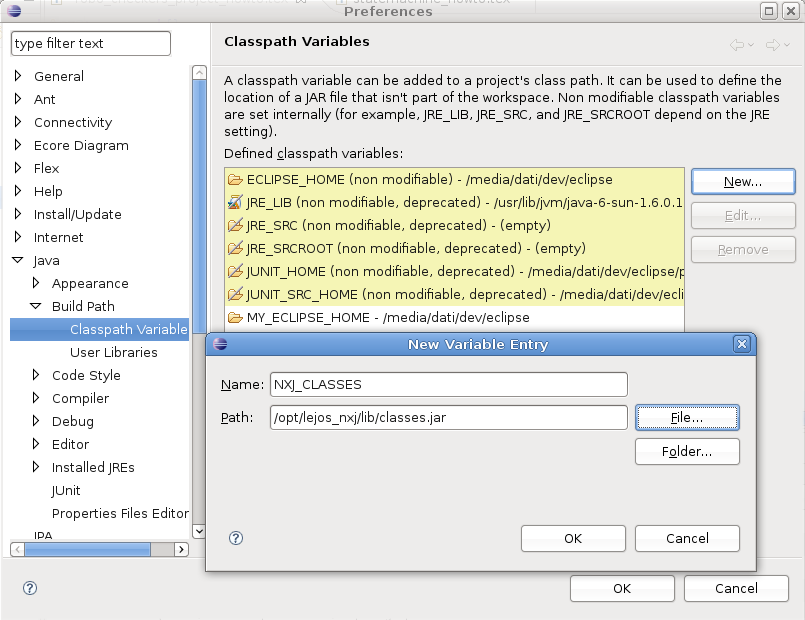
\includegraphics[scale=0.45]{img/classpath.png}
			\caption{Configurazione delle variabili d'ambiente \label{fig:classpath}}
		\end{center}
	\end{figure}
Ripetere quindi le istruzioni al passo precedente ed aggiungete altre due
variabili d'ambiente chimate \texttt{PCCOMM\_CLASSES} e
\texttt{PCTOOLS\_CLASSES} che fanno rispettivamente riferimento ai file
\emph{pccomm.jar} e \emph{pctools.jar}.
Arrivati a questo punto la configurazione dell'ambiente Eclipse � finita ed �
possibile scaricare i sorgenti del progetto.

\subsection{Checkout dal repository SVN}
Per fare il checkout dei sorgeti basta semplicemente seguire le istruzioni gi�
utilizzate in precedenta\footnote{fare riferimento al paragrafo \ref{sec:checkoutsvn}}
cambiando semplicemente l'indirizzo che risulta:
\begin{itemize}
\item \url{https://robochecker.googlecode.com/svn/roboChechersNXJ/trunk} per il
progetto base dove � presente il codice per la gestione del gioco e il
programma sequenziale;
\item \url{https://robochecker.googlecode.com/svn/roboChechers/trunk} per il
progetto della macchina a stati che far� riferimento ai sorgenti del progetto
precedente per le classi che gestiscono il gioco.
\end{itemize}

